\documentclass[12pt,a4paper]{book}
\usepackage{amsmath}
\usepackage{amssymb}
\usepackage{graphicx}
\usepackage{xcolor,float}
\usepackage{tikz}
\usepackage{qrcode}
\usepackage{fancyhdr}
\usepackage{enumitem}
\usepackage{wrapfig}
\usepackage{amsmath}
\usepackage{amssymb}
\usepackage{enumitem}
\usepackage{fancyhdr}
\usepackage{graphicx}  % For including external figures
\usepackage[left=1in,right=1in,top=1in,bottom=1in]{geometry}
\usepackage{tfrupee}


% Custom colors
\definecolor{chapterblue}{RGB}{0,175,234}

% Page geometry
\geometry{margin=1in}

% Headers and footers
\pagestyle{fancy}
\fancyhf{}
\renewcommand{\headrulewidth}{0pt}
\renewcommand{\footrulewidth}{0pt}
\fancyfoot[C]{2019-20}

% Custom chapter style
\makeatletter
\def\@makechapterhead#1{%
  \vspace*{50\p@}%
  {\parindent \z@ \raggedright \normalfont
    \ifnum \c@secnumdepth >\m@ne
      \huge\bfseries \@chapapp\space \thechapter
    \fi
    \par\nobreak
    \vskip 20\p@
    \interlinepenalty\@M
    \Huge \bfseries #1\par\nobreak
    \vskip 40\p@
  }}
\makeatother

% Custom section style
\makeatletter
\renewcommand{\section}{\@startsection{section}{1}{0mm}
  {-12pt}
  {6pt}
  {\normalfont\large\bfseries}}
\makeatother

\begin{document}

% Custom chapter heading
\thispagestyle{empty}
\begin{tikzpicture}[remember picture, overlay]
    % QR code in top center
    \node[anchor=north] at ([yshift=-1.5cm]current page.north) {
        \qrcode[height=2cm]{1062CH05}\\
        \small{1062CH05}
    };

    % Chapter heading below QR code
    \node[anchor=north] at ([yshift=-4.5cm]current page.north) {
        \begin{minipage}{\textwidth}
            \centering
            \begin{tikzpicture}
                \draw[chapterblue, line width=2pt] (0,0) -- (14,0);
                \node[left, text=chapterblue, font=\Huge\bfseries] at (11,0.7) {ARITHMETIC PROGRESSIONS};
                

            \end{tikzpicture}
        \end{minipage}
    };
\end{tikzpicture}






\vspace{7em}\textcolor{cyan}{\section{Introduction}}
You must have observed that in nature, many things follow a certain pattern, such as\\
the petals of a sunflower, the holes of a honeycomb, the grains on a maize cob, the\\
spirals on a pineapple and on a pine cone etc.

We now look for some patterns which occur in our day-to-day life. Some such
examples are :
\begin{enumerate}
   

 \item [(i)] Reena applied for a job and got selected. She 
    has been offered a job with a starting monthly
    salary of  \ 8000, with an annual increment of
     \ 500 in her salary. Her salary (in  ) for the 1st,
    2nd, 3rd, . . . years will be, respectively
    
    \hspace{2cm} 8000, \quad 8500, \quad 9000, . . . .

 \item [(ii)] The lengths of the rungs of a ladder decrease
    \\ uniformly by 2 cm from bottom to top
     \\(see Fig. 5.1). The bottom rung is 45 cm\\ in
     length. The lengths (in cm) of the 1st, 2nd,
     \\3rd, . . ., 8th rung from the bottom to the top\\
     are, respectively\\
     
     \hspace{2cm} 45, 43, 41, 39, 37, 35, 33, 31

\vspace{-12em}\hspace{22em}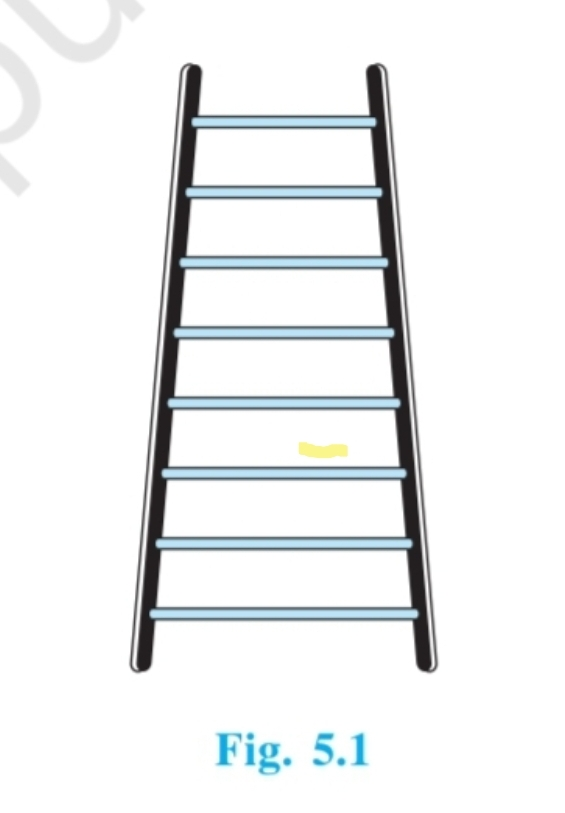
\includegraphics[width=0.2\textwidth]{Ladder.png} 


\vspace{2cm} \item [(iii)] In a savings scheme, the amount becomes $\frac{5}{4}$ times of itself after every 3 years.
     The maturity amount (in  ) of an investment of  \ 8000 after 3, 6, 9 and 12 years
     will be, respectively :
     
     \hspace{2cm} 10000, \quad 12500, \quad 15625, 19531.25
     \end{enumerate}
\newpage
% Format section titles

\noindent\textbf{2  \hfill MATHEMATICS}
% Set up headers and footers for first page on


% Normal page style for other pages
\pagestyle{plain}

% Set up paragraph spacing to match the PDF
\setlength{\parindent}{0pt}
\setlength{\parskip}{6pt}

% Define math formatting to match the PDF
\everymath{\displaystyle}

% Control the spacing to ensur

% Apply first page style to first page only

% Setup for header and footer
\pagestyle{fancy}
\fancyhf{}
\renewcommand{\headrulewidth}{0pt}
\renewcommand{\footrulewidth}{0pt}

\rfoot{2019-20}

% Roman numeral enumeration
\newcounter{romancounter}
\setcounter{romancounter}{3} % Starting from (iv)


\begin{list}{(\roman{romancounter})}{%
  \usecounter{romancounter}
  \setlength{\leftmargin}{20pt}
  \setlength{\itemsep}{15pt}
}

\item The number of unit squares in squares with side 1, 2, 3, \ldots\ units (see Fig. 5.2)
are, respectively
\begin{center}
$1^2$, $2^2$, $3^2$, \ldots\ .
\end{center}

\begin{center}
% Insert figure here
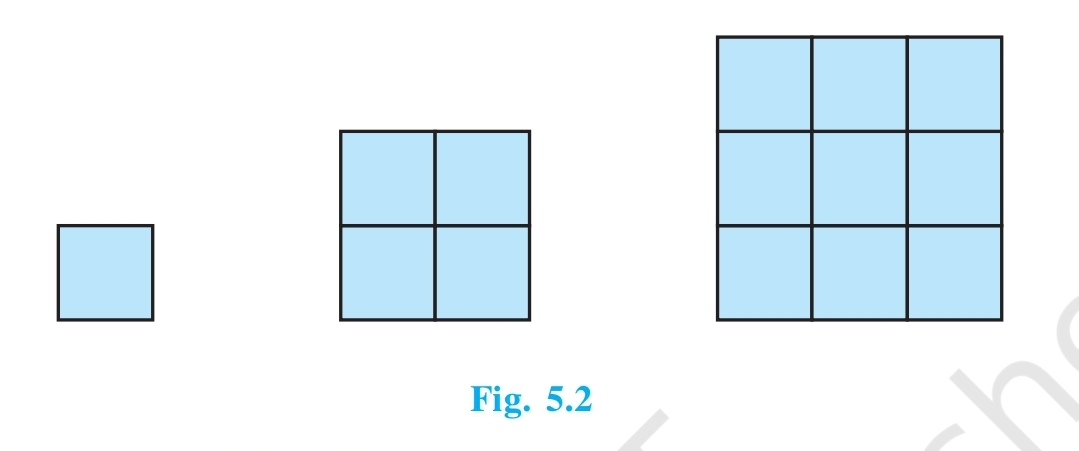
\includegraphics[width=0.3\textwidth]{Cube.png} 

\end{center}

\item Shakila puts ` 100 into her daughter's money box when she was one year old
and increased the amount by ` 50 every year. The amounts of money (in `) in the
box on the 1st, 2nd, 3rd, 4th, \ldots\ birthday were
\begin{center}
100, 150, 200, 250, \ldots, respectively.
\end{center}

\item A pair of rabbits are too young to produce in their first month. In the second, and
every subsequent month, they produce a new pair. Each new pair of rabbits
produce a new pair in their second month and in every subsequent month (see
Fig. 5.3). Assuming no rabbit dies, the number of pairs of rabbits at the start of
the 1st, 2nd, 3rd, \ldots, 6th month, respectively are:
\begin{center}
1, 1, 2, 3, 5, 8
\end{center}

\begin{center}
% Insert figure here
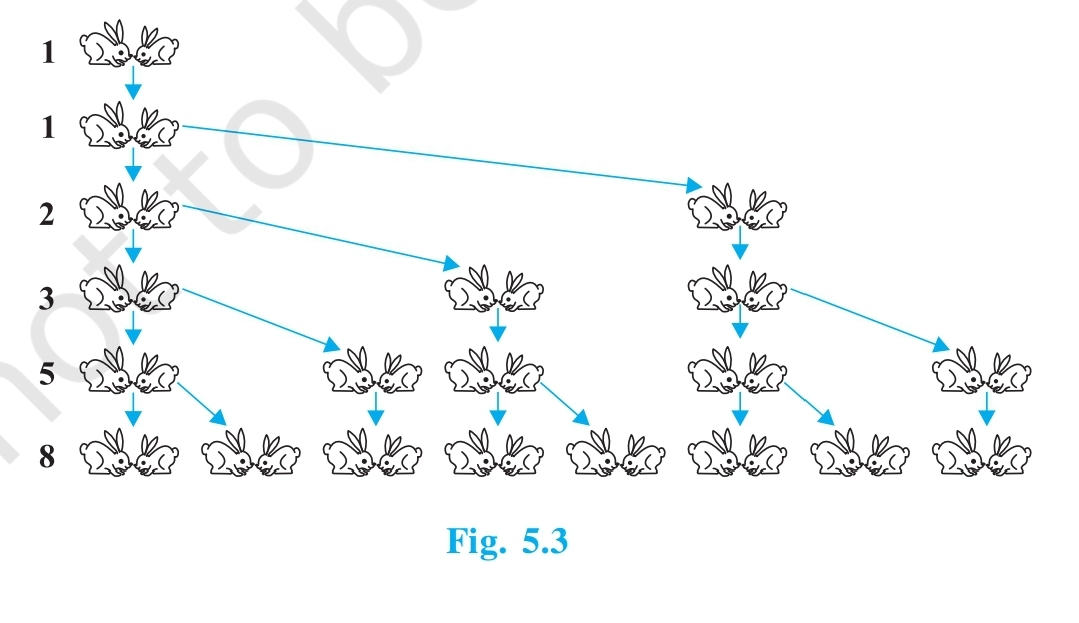
\includegraphics[width=0.55\textwidth]{Rabbit.png} 

\end{center}

\end{list}


\newpage

\noindent\textbf{3 \hfill MATHEMATICS}

\noindent In the examples above, we observe some patterns. In some, we find that the
succeeding terms are obtained by adding a fixed number, in other by multiplying
with a fixed number, in another we find that they are squares of consecutive
numbers, and so on.

In this chapter, we shall discuss one of these patterns in which succeeding terms
are obtained by adding a fixed number to the preceding terms. We shall also see how
to find their nth terms and the sum of n consecutive terms, and use this knowledge in
solving some daily life problems.



\textcolor{cyan}{\section{5.2 Arithmetic Progressions}}

\noindent Consider the following lists of numbers:
\begin{enumerate}[label=(\roman*), itemsep=1pt]
    \item 1, 2, 3, 4, \ldots
    \item 100, 70, 40, 10, \ldots
    \item $-$3, $-$2, $-$1, 0, \ldots
    \item 3, 3, 3, 3, \ldots
    \item $-$1.0, $-$1.5, $-$2.0, $-$2.5, \ldots
\end{enumerate}

Each of the numbers in the list is called a term.

Given a term, can you write the next term in each of the lists above? If so, how
will you write it? Perhaps by following a pattern or rule. Let us observe and write the
rule.

In (i), each term is 1 more than the term preceding it.

% Setup for header and footer
\pagestyle{fancy}
\fancyhf{}
\renewcommand{\headrulewidth}{0pt}
\renewcommand{\footrulewidth}{0pt}
\chead{\textbf{94 MATHEMATICS}}
\rfoot{2019-20}

% Roman numeral enumeration

\setcounter{romancounter}{3} % Starting from (iv)



\begin{list}{(\roman{romancounter})}{%
  \usecounter{romancounter}
  \setlength{\leftmargin}{20pt}
  \setlength{\itemsep}{15pt}
}

\item The number of unit squares in squares with side 1, 2, 3, \ldots\ units (see Fig. 5.2)
are, respectively
\begin{center}
$1^2$, $2^2$, $3^2$, \ldots\ .
\end{center}



\noindent\item Shakila puts 100 into her daughter's money box when she was one year old
and increased the amount by ` 50 every year. The amounts of money (in `) in the
box on the 1st, 2nd, 3rd, 4th, \ldots\ birthday were
\begin{center}
100, 150, 200, 250, \ldots, respectively.
\end{center}

\item A pair of rabbits are too young to produce in their first month. In the second, and
every subsequent month, they produce a new pair. Each new pair of rabbits
produce a new pair in their second month and in every subsequent month (see
Fig. 5.3). Assuming no rabbit dies, the number of pairs of rabbits at the start of
the 1st, 2nd, 3rd, \ldots, 6th month, respectively are:
\end{list}

\vspace{0.15cm}
\newpage

\noindent\textbf{4 \hfill MATHEMATICS}

\noindent Let us denote the first term of an AP by $a_1$, second term by $a_2$, \ldots, nth term by
$a_n$ and the common difference by $d$. Then the AP becomes
$a_1, a_2, a_3, \ldots, a_n$.

So, $a_2 - a_1 = a_3 - a_2 = \ldots = a_n - a_{n-1} = d$.

Some more examples of AP are:
\begin{enumerate}[label=(\alph*), itemsep=1pt]
    \item The heights (in cm) of some students of a school standing in a queue in the
morning assembly are 147, 148, 149, \ldots, 157.
    \item The minimum temperatures (in degree celsius) recorded for a week in the
month of January in a city, arranged in ascending order are
$-$3.1, $-$3.0, $-$2.9, $-$2.8, $-$2.7, $-$2.6, $-$2.5
    \item The balance money (in rupees) after paying 5\% of the total loan of  1000 every
month is 950, 900, 850, 800, \ldots, 50.
    \item The cash prizes (in rupees) given by a school to the toppers of Classes I to XII are,
respectively, 200, 250, 300, 350, \ldots, 750.
    \item The total savings (in rupees
    ) after every month for 10 months when  50 are saved
each month are 50, 100, 150, 200, 250, 300, 350, 400, 450, 500.
\end{enumerate}

It is left as an exercise for you to explain why each of the lists above is an AP.

You can see that
$a, a + d, a + 2d, a + 3d, \ldots$
represents an arithmetic progression where $a$ is the first term and $d$ the common
difference. This is called the general form of an AP.

Note that in examples (a) to (e) above, there are only a finite number of terms.
Such an AP is called a finite AP. Also note that each of these Arithmetic Progressions
(APs) has a last term. The APs in examples (i) to (v) in this section, are not finite APs
and so they are called infinite Arithmetic Progressions. Such APs do not have a
last term.

Now, to know about an AP, what is the minimum information that you need? Is it
enough to know the first term? Or, is it enough to know only the common difference?
You will find that you will need to know both – the first term $a$ and the common
difference $d$.

For instance if the first term $a$ is 6 and the common difference $d$ is 3, then
the AP is
$6, 9, 12, 15, \ldots$
and if $a$ is 6 and $d$ is $-$3, then the AP is
$6, 3, 0, -3, \ldots$

\newpage

\noindent\textbf{5 \hfill MATHEMATICS}

\noindent Similarly, when

$a = -7, d = -2$, the AP is $-7, -9, -11, -13, \ldots$

$a = 1.0, d = 0.1$, the AP is $1.0, 1.1, 1.2, 1.3, \ldots$

$a = 0, d = 1\frac{1}{2}$, the AP is $0, 1\frac{1}{2}, 3, 4\frac{1}{2}, 6, \ldots$

$a = 2, d = 0$, the AP is $2, 2, 2, 2, \ldots$

So, if you know what $a$ and $d$ are, you can list the AP. What about the other way
round? That is, if you are given a list of numbers can you say that it is an AP and then
find $a$ and $d$? Since $a$ is the first term, it can easily be written. We know that in an AP,
every succeeding term is obtained by adding $d$ to the preceding term. So, $d$ found by
subtracting any term from its succeeding term, i.e., the term which immediately follows
it should be same for an AP.

For example, for the list of numbers:
$6, 9, 12, 15, \ldots,$

We have $a_2 - a_1 = 9 - 6 = 3$,

$a_3 - a_2 = 12 - 9 = 3$,

$a_4 - a_3 = 15 - 12 = 3$

Here the difference of any two consecutive terms in each case is 3. So, the
given list is an AP whose first term $a$ is 6 and common difference $d$ is 3.

For the list of numbers: $6, 3, 0, -3, \ldots,$

$a_2 - a_1 = 3 - 6 = -3$

$a_3 - a_2 = 0 - 3 = -3$

$a_4 - a_3 = -3 - 0 = -3$

Similarly this is also an AP whose first term is 6 and the common difference
is $-3$.

In general, for an AP $a_1, a_2, \ldots, a_n$, we have
$d = a_{k+1} - a_k$
where $a_{k+1}$ and $a_k$ are the $(k+1)$th and the $k$th terms respectively.

To obtain $d$ in a given AP, we need not find all of $a_2 - a_1, a_3 - a_2, a_4 - a_3, \ldots$.
It is enough to find only one of them.

Consider the list of numbers $1, 1, 2, 3, 5, \ldots$. By looking at it, you can tell that the
difference between any two consecutive terms is not the same. So, this is not an AP.

\end{document}
